% !TEX root = ../main.tex

\chapter{Propriedades da transformada de Fourier}
\section{Propriedades}
\begin{teo}[Linearidade ou superposição]\label{prop_linear}
Dadas duas funções $f(t)$ e $g(t)$ com transformadas de Fourier $F(w)$ e $G(w)$, respectivamente, e $\alpha$ e $\beta$ duas constantes reais ou complexas, então
\begin{equation}
\mathcal{F}\left\{\alpha f(t)+\beta g(t)\right\}=\alpha \mathcal{F}\{ f(t)\}+\beta\mathcal{F}\{ g(t)\}=\alpha F(w)+\beta G(w)
\end{equation}
\end{teo}
\begin{proof}
O resultado é direto da linearidade da integral:
\begin{eqnarray*}
\mathcal{F}\left\{\alpha f(t)+\beta g(t)\right\}&=&\int_{-\infty}^\infty \left(\alpha f(t)+\beta g(t)\right) e^{-iwt}dt \\
&=&\int_{-\infty}^\infty \alpha f(t)e^{-iwt}dt+\int_{-\infty}^\infty \beta g(t) e^{-iwt}dt \\
&=&\alpha\int_{-\infty}^\infty  f(t)e^{-iwt}dt+\beta\int_{-\infty}^\infty  g(t) e^{-iwt}dt \\
&=&\alpha F(w)+\beta G(w)
\end{eqnarray*}
\end{proof}
\begin{ex}As transformadas das funções $f(t)=e^{-|t|}$ e $g(t)=\frac{1}{2\sqrt{\pi}}e^{-\frac{t^2}{4}}$ são $F(w)=\frac{2}{w^2+1}$ e $G(w)=e^{-w^2}$, respectivamente. Logo,
\begin{equation}
\mathcal{F}\left\{5 f(t)-3 g(t)\right\}=5 \frac{2}{w^2+1}-3e^{-w^2}
\end{equation}
\end{ex}
\begin{teo}[Transformada da derivada]{\label{prop_der}} Dada uma função diferenciável $f(t)$ tal que 
\begin{equation}\lim_{t\to \pm \infty}f(t)=0
\end{equation}
e sua transformada de Fourier $F(w)$, então
\begin{equation}
\mathcal{F}\{f'(t)\}=iw F(w)
\end{equation}
\end{teo}
\begin{proof}
De fato, usando integração por partes, temos
\begin{eqnarray*}
\mathcal{F}\left\{f'(t)\right\}&=&\int_{-\infty}^\infty  f'(t)e^{-iwt}dt \\
&=&\left[f(t)e^{-iwt}\right]_{-\infty}^\infty- \int_{-\infty}^\infty  -iw f(t)e^{-iwt}dt \\
&=&iw\int_{-\infty}^\infty   f(t)e^{-iwt}dt \\
&=&iwF(w) 
\end{eqnarray*}
\end{proof}
\begin{obs}Essa propriedade reflete o fato de que a transformada de Fourier decompõe a função $f(t)$ em funções do tipo $e^{iwt}$ cuja derivada é $iwe^{iwt}$. De fato, esta propriedade poderia ter sido deduzida a partir da representação de $f(t)$ em sua integral de Fourier, isto é:
\begin{equation}
f(t)=\frac{1}{2\pi}\int_{-\infty}^\infty F(w)e^{iwt}dw.
\end{equation}
Diferenciando em $t$, obtemos
\begin{equation}
f'(t)=\frac{1}{2\pi}\int_{-\infty}^\infty F(w)iwe^{iwt}dw=\frac{1}{2\pi}\int_{-\infty}^\infty \left[iwF(w)\right]e^{iwt}dw.
\end{equation}
\end{obs}
\begin{ex}{\label{ex_exp_t2}}Considere a função $f(t)=e^{-at^2}$, $a>0$, e sua transformada de Fourier (ver exercício \ref{Exer_trans_exp_t2} da página \pageref{Exer_trans_exp_t2}):
\begin{equation}
F(w)=\frac{\sqrt{\pi}}{\sqrt{a}}e^{-\frac{w^2}{4a}}
\end{equation}
Usando a propriedade \ref{prop_der}, a transformada de Fourier da derivada $f'(t)=-2 a t e^{-at^2}$ é dada por:
\begin{equation}
\mathcal{F}\{-2 a t e^{-at^2} \}=iwF(w)=iw\frac{\sqrt{\pi}}{\sqrt{a}}e^{-\frac{w^2}{4a}}.
\end{equation}
Usando a linearidade, encontramos a transformada de Fourier da função $t e^{-at^2}$:
\begin{equation}
\mathcal{F}\{  t e^{-at^2} \}=-iw\frac{\sqrt{\pi}}{2a\sqrt{a}}e^{-\frac{w^2}{4a}}.
\end{equation}
Compare com o exercício \ref{exer_te_t2} da página \pageref{exer_te_t2}.
\end{ex}
\begin{obs}As derivadas de ordem superior são calculadas a partir da propriedade \ref{prop_der}:
\begin{eqnarray*}
\mathcal{F}\{f''(t)\}&=&\mathcal{F}\left\{\frac{d}{dt}\left(f'(t)\right)\right\}\\
&=&iw\mathcal{F}\left\{f'(t)\right\}\\
&=&(iw)^2\mathcal{F}\left\{f(t)\right\}\\
&=&(iw)^2F(w).
\end{eqnarray*}
De modo geral,
\begin{eqnarray*}
\mathcal{F}\{f^{(n)}(t)\}=(iw)^nF(w).
\end{eqnarray*}
\end{obs}
\begin{teo}[Deslocamento no eixo $w$]\label{prop_desl_w} Dada uma função $f(t)$ e sua transformada de Fourier $F(w)$, então
\begin{equation}
\mathcal{F}\left\{e^{at}f(t)\right\}=F(w+ia).
\end{equation}
\end{teo}
\begin{proof}
De fato,
\begin{eqnarray*}
\mathcal{F}\left\{e^{at}f(t)\right\}&=&\int_{-\infty}^\infty  f(t)e^{at}e^{-iwt}dt \\
&=&\int_{-\infty}^\infty   f(t)e^{(a-iw)t}dt \\
&=&\int_{-\infty}^\infty   f(t)e^{-i(ia+w)t}dt \\
&=&F(w+ia) 
\end{eqnarray*}
\end{proof}
\begin{ex} Do exemplo \ref{ex_exp_t2} temos que a transformada de Fourier da função $f(t)=t e^{-at^2}$, $a>0$, é dada por
\begin{equation}
F(w)=-iw\frac{\sqrt{\pi}}{2a\sqrt{a}}e^{-\frac{w^2}{4a}}.
\end{equation}
Logo, a transformada $G(w)$ da função $g(t)=t e^{bt-at^2}$, $b>0$, é dada por
\begin{eqnarray*}
G(w)=\mathcal{F}\left\{t e^{bt-at^2}\right\}&=&\mathcal{F}\left\{e^{bt}t e^{-at^2}\right\}\\
&=&F(w+ib)\\
&=&-i(w+ib)\frac{\sqrt{\pi}}{2a\sqrt{a}}e^{-\frac{(w+ib)^2}{4a}}\\
&=&(b-iw)\frac{\sqrt{\pi}}{2a\sqrt{a}}e^{-\frac{w^2+2wib-b^2}{4a}}\\
&=&\sqrt{w^2+b^2}e^{-i\arctan\left(\frac{w}{b}\right)}\frac{\sqrt{\pi}}{2a\sqrt{a}}e^{-\frac{w^2-b^2}{4a}}e^{-i\left(\frac{wb}{2a}\right)}\\
&=&\sqrt{w^2+b^2}\frac{\sqrt{\pi}}{2a\sqrt{a}}e^{-\frac{w^2-b^2}{4a}}e^{-i\left(\frac{wb}{2a}+\arctan\left(\frac{w}{b}\right)\right)}\\
&=&|G(w)|e^{i\phi(w)},
\end{eqnarray*}
onde
\begin{eqnarray*}
|G(w)|=\frac{\sqrt{\pi}}{2a\sqrt{a}}e^{-\frac{b^2}{4a}}\sqrt{w^2+b^2}e^{-\frac{w^2}{4a}}\qquad\hbox{ e }\qquad \phi(w)=-\left(\frac{wb}{2a}+\arctan\left(\frac{w}{b}\right)\right)
\end{eqnarray*}
Veja os diagramas de espectro de $G(w)$ quando $a=b=1$ na figura \ref{diag_espec_trans_4}.
\begin{figure}[!ht]
\begin{center}
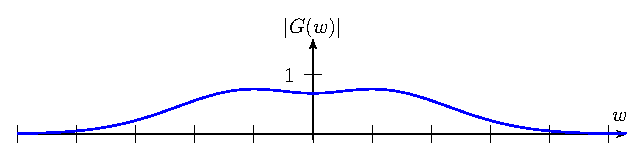
\includegraphics[width=\textwidth]{cap_propriedades_transformada/pics/figura_2}\vspace{10pt}
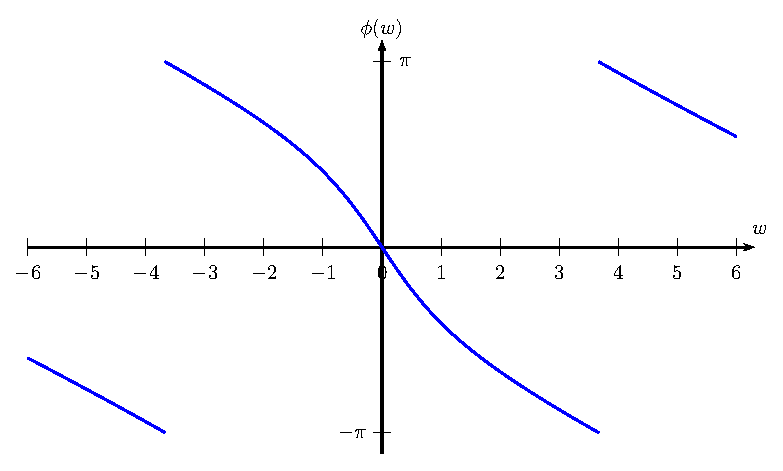
\includegraphics[width=\textwidth]{cap_propriedades_transformada/pics/figura_3}
[width=textwidth]\end{center}
\caption{\label{diag_espec_trans_4}}
\end{figure}
\end{ex}

\begin{teo}[Deslocamento no eixo $t$]\label{prop_desl_t} Dada uma função $f(t)$ e sua transformada de Fourier $F(w)$, então
\begin{equation}
\mathcal{F}\left\{f(t-a)\right\}=e^{-iaw}F(w).
\end{equation}
\end{teo}
\begin{proof}
De fato,
\begin{eqnarray*}
\mathcal{F}\left\{f(t-a)\right\}&=&\int_{-\infty}^\infty  f(t-a)e^{-iwt}dt \\
&=&\int_{-\infty}^\infty  f(s)e^{-iw(s+a)}ds \\
&=&\int_{-\infty}^\infty  f(s)e^{-iwa}e^{-iws}ds \\
&=&e^{-iwa}\int_{-\infty}^\infty  f(s)e^{-iws}ds \\
&=&e^{-iaw}F(w)
\end{eqnarray*}
\end{proof}
\begin{ex}{\label{ex_desloc_tempo}} Do exemplo \ref{ex_Transf_1} da página \pageref{ex_Transf_1} temos que a transformada de Fourier da função $f(t)=e^{-|t|}$ é dada por $F(w)=\frac{2}{w^2+1}$. Logo, a transformada de Fourier da função $g(t)=e^{-|t-2|}$ é
\begin{equation}
G(w)=\frac{2}{w^2+1}e^{-2iw}
\end{equation}
\end{ex}
\begin{obs} Um deslocamento real no tempo não altera o módulo da transformada de Fourier, pois $|e^{-iaw}|=1$ sempre que $a$ e $w$ são reais.
\end{obs}
\begin{teo}[Transformada da integral]\label{prop_int} Dada uma função integrável $f(t)$ tal que sua transformada de Fourier $F(w)$ satisfaça $F(0)=0$, então
\begin{equation}
\mathcal{F}\left\{\int_{-\infty}^t f(\tau)d\tau \right\}=\frac{1}{iw}F(w).
\end{equation}
\end{teo}
\begin{proof}
Definimos $g(t)=\int_{-\infty}^t f(\tau)d\tau$ e, usando o teorema fundamental do cálculo, temos $g'(t)=f(t)$. Aplicamos a transformada de Fourier na igualdade e temos:
\begin{equation}
\mathcal{F}\{g'(t)\}=\mathcal{F}\{f(t)\},
\end{equation}
ou seja,
\begin{equation}
\mathcal{F}\{g'(t)\}=F(w).
\end{equation}
Observe que
\begin{equation}
\lim_{t\to\infty} g(t)=\int_{-\infty}^\infty f(\tau)d\tau=\int_{-\infty}^\infty f(\tau)e^{i\cdot 0 \cdot \tau}d\tau=F(0)=0
\end{equation}
e
\begin{equation}
\lim_{t\to-\infty} g(t)=\int_{-\infty}^{-\infty} f(\tau)d\tau=0,
\end{equation}
portanto, podemos usar a propriedade \ref{prop_der} da transformada de Fourier da derivada e obter:
\begin{equation}
\mathcal{F}\{g'(t)\}=iw \mathcal{F}\{g(t)\}.
\end{equation}
Assim,
\begin{equation}
F(w)=iw \mathcal{F}\left\{\int_{-\infty}^t f(\tau)d\tau\right\}.
\end{equation}
Portanto,
\begin{equation}
\mathcal{F}\left\{\int_{-\infty}^t f(\tau)d\tau\right\}=\frac{1}{iw}F(w).
\end{equation}
\end{proof}
\begin{teo}[Teorema da modulação]\label{prop_mod}  Dada uma função $f(t)$ e sua transformada de Fourier $F(w)$, então
\begin{equation}
\mathcal{F}\left\{f(t)\cos(w_0t) \right\}=\frac{1}{2}F(w-w_0)+\frac{1}{2}F(w+w_0),
\end{equation}
para $w_0\in\mathbb{R}$.
\end{teo}
\begin{proof}
De fato,
\begin{eqnarray*}
\mathcal{F}\left\{f(t)\cos(w_0t) \right\}&=&\mathcal{F}\left\{f(t)\left(\frac{e^{iw_0t}+e^{-iw_0t}}{2} \right)\right\} \\
&=&\int_{-\infty}^\infty f(t)\frac{e^{iw_0t}+e^{-iw_0t}}{2}e^{-iwt}dt  \\
&=&\frac{1}{2}\int_{-\infty}^\infty f(t)e^{-i(w-w_0)t}dt+\frac{1}{2}  \int_{-\infty}^\infty f(t)e^{-i(w_0+w)t}dt\\
&=&\frac{1}{2}F(w-w_0)+\frac{1}{2}F(w+w_0)
\end{eqnarray*}
\end{proof}
\begin{ex}{\label{ex_prop_trans_1.0}}Considere a função $f(t)=\cos(w_0t) e^{-a|t|}$, $a>0$. Podemos obter a transformada de Fourier de $f(t)$ a partir da transformada de Fourier da função $g(t)=e^{-a|t|}$. Basta aplicar o teorema da modulação à função $g(t)$, cuja transformada de Fourier é dada por $G(w)=\frac{2a}{w^2+a^2}$:
\begin{eqnarray*}
\mathcal{F}\left\{g(t)\cos(w_0t) \right\}&=&\frac{1}{2}G(w-w_0)+\frac{1}{2}G(w+w_0)\\
&=&\frac{1}{2}\frac{2a}{(w-w_0)^2+a^2}+\frac{1}{2}\frac{2a}{(w+w_0)^2+a^2}\\
&=&\frac{a}{(w-w_0)^2+a^2}+\frac{a}{(w+w_0)^2+a^2}
\end{eqnarray*}
\end{ex}
\begin{teo} [Teorema da convolução]\label{prop_teo_conv} Dadas duas funções $f_1(t)$ e $f_2(t)$ com suas respectivas transformadas de Fourier, $F_1(w)$ e $F_2(w)$, então
\begin{itemize}
\item[a)] (Convolução no tempo)
\begin{equation}\mathcal{F}\{(f_1*f_2)(t)\}=F_1(w)F_2(w),\end{equation}
\item[b)] (Convolução na frequência)
\begin{equation}(F_1*F_2)(w)=2\pi\mathcal{F}\{f_1(t)f_2(t)\}\end{equation}
ou 
\begin{equation}\mathcal{F}^{-1}\{(F_1*F_2)(w)\}=2\pi f_1(t)f_2(t),\end{equation}
\end{itemize}
onde $*$ indica a convolução de duas funções:
\begin{equation}
(f_1*f_2)(t)=\int_{-\infty}^\infty f_1(\tau)f_2(t-\tau)d\tau
\end{equation}
\end{teo}
\begin{proof}
\begin{itemize}
\item[a)] Usando as definições de transformada de Fourier e convolução de duas funções, temos:
\begin{eqnarray}
\nonumber \mathcal{F}\{(f_1*f_2)(t)\}&=&\int_{-\infty}^\infty (f_1*f_2)(t)e^{-iwt}dt\\
\nonumber &=&\int_{-\infty}^\infty \left(\int_{-\infty}^\infty f_1(\tau)f_2(t-\tau)d\tau\right)e^{-iwt}dt\\
&=&\int_{-\infty}^\infty \left[f_1(\tau) \int_{-\infty}^\infty f_2(t-\tau)e^{-iwt}dt\right]d\tau  {\label{eq_teo_conv}}
\end{eqnarray}
Uma das integrais pode ser calculada fazendo uma mudança de variável:
\begin{eqnarray}
\nonumber \int_{-\infty}^\infty f_2(t-\tau)e^{-iwt}dt&=&\int_{-\infty}^\infty f_2(s)e^{-iw(s+\tau)}ds \\
\nonumber &=&e^{-iw\tau}\int_{-\infty}^\infty f_2(s)e^{-iws}ds \\
&=&e^{-iw\tau}F_2(w) {\label{eq_teo_conv_1}}
\end{eqnarray}
Substituindo a equação (\ref{eq_teo_conv_1}) na equação (\ref{eq_teo_conv}), temos
\begin{eqnarray*}
\mathcal{F}\{(f_1*f_2)(t)\}&=&\int_{-\infty}^\infty \left[f_1(\tau) \int_{-\infty}^\infty f_2(t-\tau)e^{-iwt}dt\right]d\tau\\
&=&\int_{-\infty}^\infty \left[f_1(\tau) e^{-iw\tau}F_2(w)\right]d\tau\\
&=&F_2(w)\int_{-\infty}^\infty \left[f_1(\tau) e^{-iw\tau}\right]d\tau\\
&=&F_1(w)F_2(w)
\end{eqnarray*}
\item[b)] Analogamente, usando as definições, temos:
\begin{eqnarray}
\nonumber\mathcal{F}^{-1}\{(F_1*F_2)(w)\}&=&\frac{1}{2\pi}\int_{-\infty}^\infty (F_1*F_2)(w)e^{iwt}dw\\
\nonumber &=&\frac{1}{2\pi}\int_{-\infty}^\infty \left(\int_{-\infty}^\infty F_1(v)F_2(w-v)dv \right)e^{iwt}dw\\
&=&\frac{1}{2\pi}\int_{-\infty}^\infty\left[ F_1(v) \int_{-\infty}^\infty F_2(w-v)e^{iwt}dw \right]dv {\label{eq_teo_conv_2}}
\end{eqnarray}
Também,
\begin{eqnarray}
\nonumber \int_{-\infty}^\infty F_2(w-v)e^{iwt}dw&=&\int_{-\infty}^\infty F_2(y)e^{i(y+v)t}dy \\
\nonumber &=&e^{ivt}\int_{-\infty}^\infty F_2(y)e^{iyt}dy \\
&=&2\pi e^{ivt}f_2(t) {\label{eq_teo_conv_3}}
\end{eqnarray}
Substituindo a equação (\ref{eq_teo_conv_3}) na equação (\ref{eq_teo_conv_2}), temos
\begin{eqnarray*}
\mathcal{F}^{-1}\{(F_1*F_2)(w)\}&=&\frac{1}{2\pi}\int_{-\infty}^\infty\left[ F_1(v) \int_{-\infty}^\infty F_2(w-v)e^{iwt}dw \right]dv\\
&=&\frac{1}{2\pi}\int_{-\infty}^\infty  F_1(v) e^{ivt} 2\pi f_2(t) dv\\
&=&f_2(t)\int_{-\infty}^\infty F_1(v) e^{ivt} dv\\
&=&2\pi f_1(t)f_2(t)
\end{eqnarray*}
\end{itemize}
\end{proof}
\begin{ex}Considere as funções $f(t)=te^{-t^2}$ e $g(t)=e^{-a|t|}$, $a>0$ e suas respectivas transformadas de Fourier $F(w)=-iw\frac{\sqrt{\pi}}{2}e^{-\frac{w^2}{4}}$ e $G(w)=\frac{2a}{w^2+a^2}$. A transformada de Fourier da função 
\begin{equation}
h(t)=\int_{-\infty}^\infty f(t-\tau)g(\tau)d\tau=\int_{-\infty}^\infty (t-\tau)e^{-(t-\tau)^2}e^{-a|\tau|}d\tau
\end{equation}
é calculada usando o teorema da convolução e é dada por
\begin{equation}
H(w)=F(w)G(w)=-iwa\frac{\sqrt{\pi}}{w^2+a^2}e^{-\frac{w^2}{4}}
\end{equation}
\end{ex}
\begin{teo}[Conjugação] \label{prop_conj}Dada uma função real $f(t)$ e sua transformada de Fourier $F(w)$, então
\begin{equation}
\overline{F(w)}=F(-w)
\end{equation}
\end{teo}
\begin{proof}
De fato,
\begin{eqnarray*}
\overline{F(w)}&=&\overline{\int_{-\infty}^\infty f(t)e^{-iwt}dt}\\
&=&\int_{-\infty}^\infty f(t)\overline{e^{-iwt}}dt,\quad \hbox{pois}\ \ \overline{f(t)}=f(t) \\
&=&\int_{-\infty}^\infty f(t)e^{iwt}dt\\
&=&\int_{-\infty}^\infty f(t)e^{-i(-w)t}dt\\
&=&F(-w)
\end{eqnarray*}
\end{proof}
\begin{obs} Se $f(t)$ não é uma função real, esta propriedade não se aplica.
\end{obs}
\begin{ex}Considere as funções $f(t)=te^{-t^2}$ e sua transformada de Fourier $F(w)=-iw\frac{\sqrt{\pi}}{2}e^{-\frac{w^2}{4}}$. Então,
\begin{equation}
F(-w)=iw\frac{\sqrt{\pi}}{2}e^{-\frac{w^2}{4}}
\end{equation}
e
\begin{equation}
\overline{F(w)}=\overline{-iw\frac{\sqrt{\pi}}{2}e^{-\frac{w^2}{4}}}=iw\frac{\sqrt{\pi}}{2}e^{-\frac{w^2}{4}}.
\end{equation}
\end{ex}
\begin{teo}[Inversão temporal]\label{prop_inv_temp} Dada uma função $f(t)$ e sua transformada de Fourier $F(w)$, então \begin{equation}\mathcal{F}\left\{f(-t)\right\}=F(-w).\end{equation}
\end{teo}
\begin{proof}
\begin{eqnarray*}
\mathcal{F}\left\{f(-t)\right\}=\int_{-\infty}^\infty f(-t) e^{-iwt}dt
\end{eqnarray*}
procedemos com a mudança de variáveis $\tau=-t$:
\begin{eqnarray*}
\mathcal{F}\left\{f(-t)\right\}&=&\int_{-\infty}^\infty f(-t) e^{-iwt}dt\\
&=&\int_{\infty}^{-\infty} f(\tau) e^{iw\tau}(-d\tau) \\
&=&\int_{-\infty}^{\infty} f(\tau) e^{iw\tau}d\tau \\
&=&\int_{-\infty}^{\infty} f(\tau) e^{-i(-w)\tau}d\tau \\
&=&F(-w)
\end{eqnarray*}
\end{proof}
\begin{teo}[Simetria ou dualidade]\label{prop_sim_dua} Dada uma função $f(t)$ e sua transformada de Fourier $F(w)$, então 
\begin{equation}
f(-w)=\frac{1}{2\pi}\mathcal{F}\{F(t)\}
\end{equation}
\end{teo}
\begin{proof} Da definição de transformada de Fourier, temos
\begin{equation}
f(t)=\frac{1}{2\pi}\int_{-\infty}^{\infty} F(w)e^{iwt}dw
\end{equation}
Podemos trocas $t$ e $w$ e calcular $f(w)$ em função de $F(t)$:
\begin{equation}
f(w)=\frac{1}{2\pi}\int_{-\infty}^{\infty} F(t)e^{itw}dt.
\end{equation}
Ou seja, 
\begin{equation}
f(-w)=\frac{1}{2\pi}\int_{-\infty}^{\infty} F(t)e^{-itw}dt=\frac{1}{2\pi}\mathcal{F}\{F(t)\}.
\end{equation}
\end{proof}
\begin{teo}[Mudança de escala]\label{prop_mud_esc} Dada uma função $f(t)$ e sua transformada de Fourier $F(w)$, então 
\begin{equation}
\mathcal{F}\{f(at)\}=\frac{1}{|a|}F\left(\frac{w}{a}\right),~~ \forall a\neq 0.
\end{equation}
\end{teo}
\begin{proof} Da definição de transformada de Fourier, temos
\begin{equation}
\mathcal{F}\{f(at)\}=\int_{-\infty}^{\infty} f(at)e^{-iwt}dt
\end{equation}
Fazendo a mudança $\tau= at$, distinguindo dois casos: $a>0$ e $a<0$.
Para o caso $a>0$, temos:
\begin{eqnarray*}
\mathcal{F}\{f(at)\}&=&\int_{-\infty}^{\infty} f(at)e^{-iwt}dt\\
&=&\int_{-\infty}^{\infty} f(\tau)e^{-\frac{iw\tau}{a}}\frac{d\tau}{a}\\
&=&\frac{1}{a}\int_{-\infty}^{\infty} f(\tau)e^{-\frac{iw\tau}{a}}d\tau
\end{eqnarray*}
Para o caso $a<0$, temos:
\begin{eqnarray*}
\mathcal{F}\{f(at)\}&=&\int_{-\infty}^{\infty} f(at)e^{-iwt}dt\\
&=&\int_{\infty}^{-\infty} f(\tau)e^{-\frac{iw\tau}{a}}\frac{d\tau}{a}\\
&=&-\frac{1}{a}\int_{-\infty}^{\infty} f(\tau)e^{-\frac{iw\tau}{a}}d\tau
\end{eqnarray*}
Em ambos os casos, temos:
\begin{eqnarray*}
\mathcal{F}\{f(at)\}&=&\frac{1}{|a|}\int_{-\infty}^{\infty} f(\tau)e^{-\frac{iw\tau}{a}}d\tau\\
&=&\frac{1}{|a|}F\left(\frac{w}{a}\right)
\end{eqnarray*}
\end{proof}
\begin{obs} A propriedade da inversão temporal (propriedade \ref{prop_inv_temp}) é um caso particular desta propriedade quando $a=-1$.
\end{obs}
\subsection*{Exercícios}
\begin{exer}O diagrama de magnitudes da transformada de Fourier $F(w)$ de uma função $f(t)$ é dado na figura abaixo. Esboce o diagrama de magnitudes da transformada de Fourier da função $f'(t)$. 
%\begin{figure}[!ht]
\begin{center} 
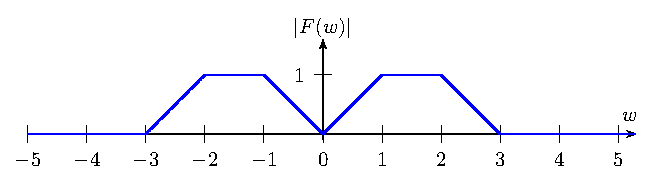
\includegraphics{cap_propriedades_transformada/pics/figura_1}\end{center}
%\caption{\label{fig_graf_1}}
%\end{figure}
\end{exer}
\begin{exer}Faça o diagrama de espectro da transformada de Fourier do exemplo \ref{ex_desloc_tempo} da página \pageref{ex_desloc_tempo}.
\end{exer}
\begin{resp}Ver figura abaixo.
\begin{center}
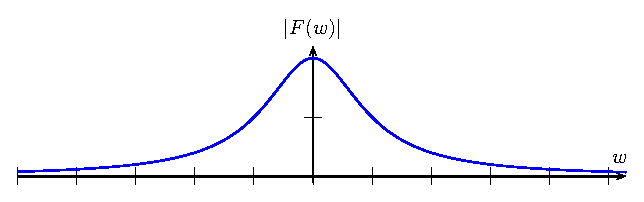
\includegraphics{cap_propriedades_transformada/pics/figura_11}
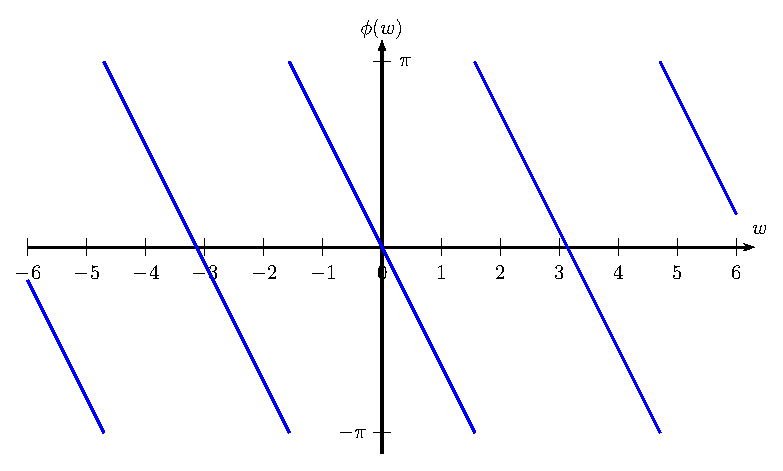
\includegraphics{cap_propriedades_transformada/pics/figura_12}\end{center}
\end{resp}
\begin{exer} Em geral não é verdade que módulo da soma é igual a soma dos módulos, isto é, $|x+y|=|x|+|y|$, $x,y\in\mathbb{C}$.
\begin{itemize}
\item[a)] Encontre um caso particular onde $|x+y|=|x|+|y|$ com $|x|\neq 0$ e $|y|\neq 0$.
\item[b)] Encontre um caso particular onde $|x+y|=0$ com $|x|\neq 0$ e $|y|\neq 0$. Mostre que, nesse caso, $x=-y$.
\item[c)] Encontre um caso particular onde $|x+y|=1$ com $|x|=|y|=1$.
\item[d)] Mostre que $|x+y|=|x|+|y|$ sempre que $xy=0$.
\end{itemize}
Observe que não é possível, em geral, conhecer o diagrama de magnitudes da soma de duas funções, $F(w)$ e $G(w)$, conhecendo apenas seus diagramas de magnitudes. As fases precisam ser levadas em conta. Um exceção é quando, para todos $w$, ou $F(w)=0$ ou $G(w)=0$.
\end{exer}
\begin{exer}{\label{ex_mod_sin}}Mostre que, dada uma função $f(t)$ e sua transformada de Fourier $F(w)$, então
\begin{equation}
\mathcal{F}\left\{f(t)\sen(w_0t) \right\}=\frac{i}{2}F(w+w_0)-\frac{i}{2 }F(w-w_0),
\end{equation}
para $w_0\in\mathbb{R}$.
\end{exer}
\begin{exer}Considere uma função real $f(t)$ tal que o diagrama de magnitude é dado na figura abaixo. 
\begin{center}
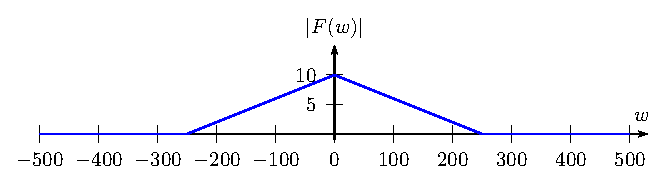
\includegraphics{cap_propriedades_transformada/pics/figura_13}\end{center}
\begin{itemize}
\item[a)] Trace o diagrama de magnitude do espectro de $g(t)=f(t-a)$ onde $a$ é uma constante real.
\item[b)] Trace o diagrama de magnitude do espectro de $g(t)=f(2t)$.
\item[c)] Trace o diagrama de magnitude do espectro de $g(t)=f(-t)$.
\item[d)] Trace o diagrama de magnitude do espectro de $g(t)=3f(t)$.
\item[e)] Trace o diagrama de magnitude do espectro de $g(t)=f(t)\cos(1000t)$.
\item[f)] Trace o diagrama de magnitude do espectro de $g(t)=f(t)\cos^2(1000t)$.
\item[g)] Trace o diagrama de magnitude do espectro de $g(t)=f(t)\sen(1000t)$.
\item[h)] Trace o diagrama de magnitude do espectro de $g(t)=f(t)|\sen(1000t)|$. [Dica: Use a expansão em Série de Fourier do retificador de onda completa\footnote{$|\sen(x)|=\frac{2}{\pi}-\frac{4}{\pi}\left(\frac{\cos(2x)}{1\cdot 3}+\frac{\cos(4x)}{3\cdot 5}+\frac{\cos(6x)}{5\cdot 7}+\cdots\right)$}]
\item[i)] Trace o diagrama de magnitude do espectro de $g(t)=f'(t)$.
\item[j)] Trace o diagrama de magnitude do espectro de $g(t)=f(t)\ast f(t)$.
\item[k)] Calcule o valor da energia do sinal dada por \begin{equation}\int_{-\infty}^\infty f(t)^2dt.\end{equation}
\item[l)] Calcule o módulo do valor médio do sinal dado por \begin{equation}\left|\int_{-\infty}^\infty f(t)dt\right|.\end{equation}
\end{itemize}
 \end{exer}
\begin{resp}
\begin{itemize}
\item[a)]
 \begin{eqnarray*}
\mathcal{F}\left\{g(t)\right\}&=&\mathcal{F}\left\{f(t-a)\right\}=\mathcal{F}\left\{f(t)\right\}e^{-iaw}\\
\left|\mathcal{F}\left\{g(t)\right\}\right|&=&|F(w)|~|e^{-iaw}|=|F(w)|
\end{eqnarray*}
Onde se usou a propriedade \ref{prop_desl_t}
Logo o diagrama de magnitude é o mesmo do de $f(t)$.
\item[b)] 
 \begin{eqnarray*}
\mathcal{F}\left\{g(t)\right\}&=&\mathcal{F}\left\{f(2t)\right\}=\frac{1}{2}F\left(\frac{w}{2}\right)\\
\left|\mathcal{F}\left\{g(t)\right\}\right|&=&\frac{1}{2}\left|F\left(\frac{w}{2}\right)\right|.
\end{eqnarray*}
Onde se usou a propriedade \ref{prop_mud_esc}.
\begin{center}
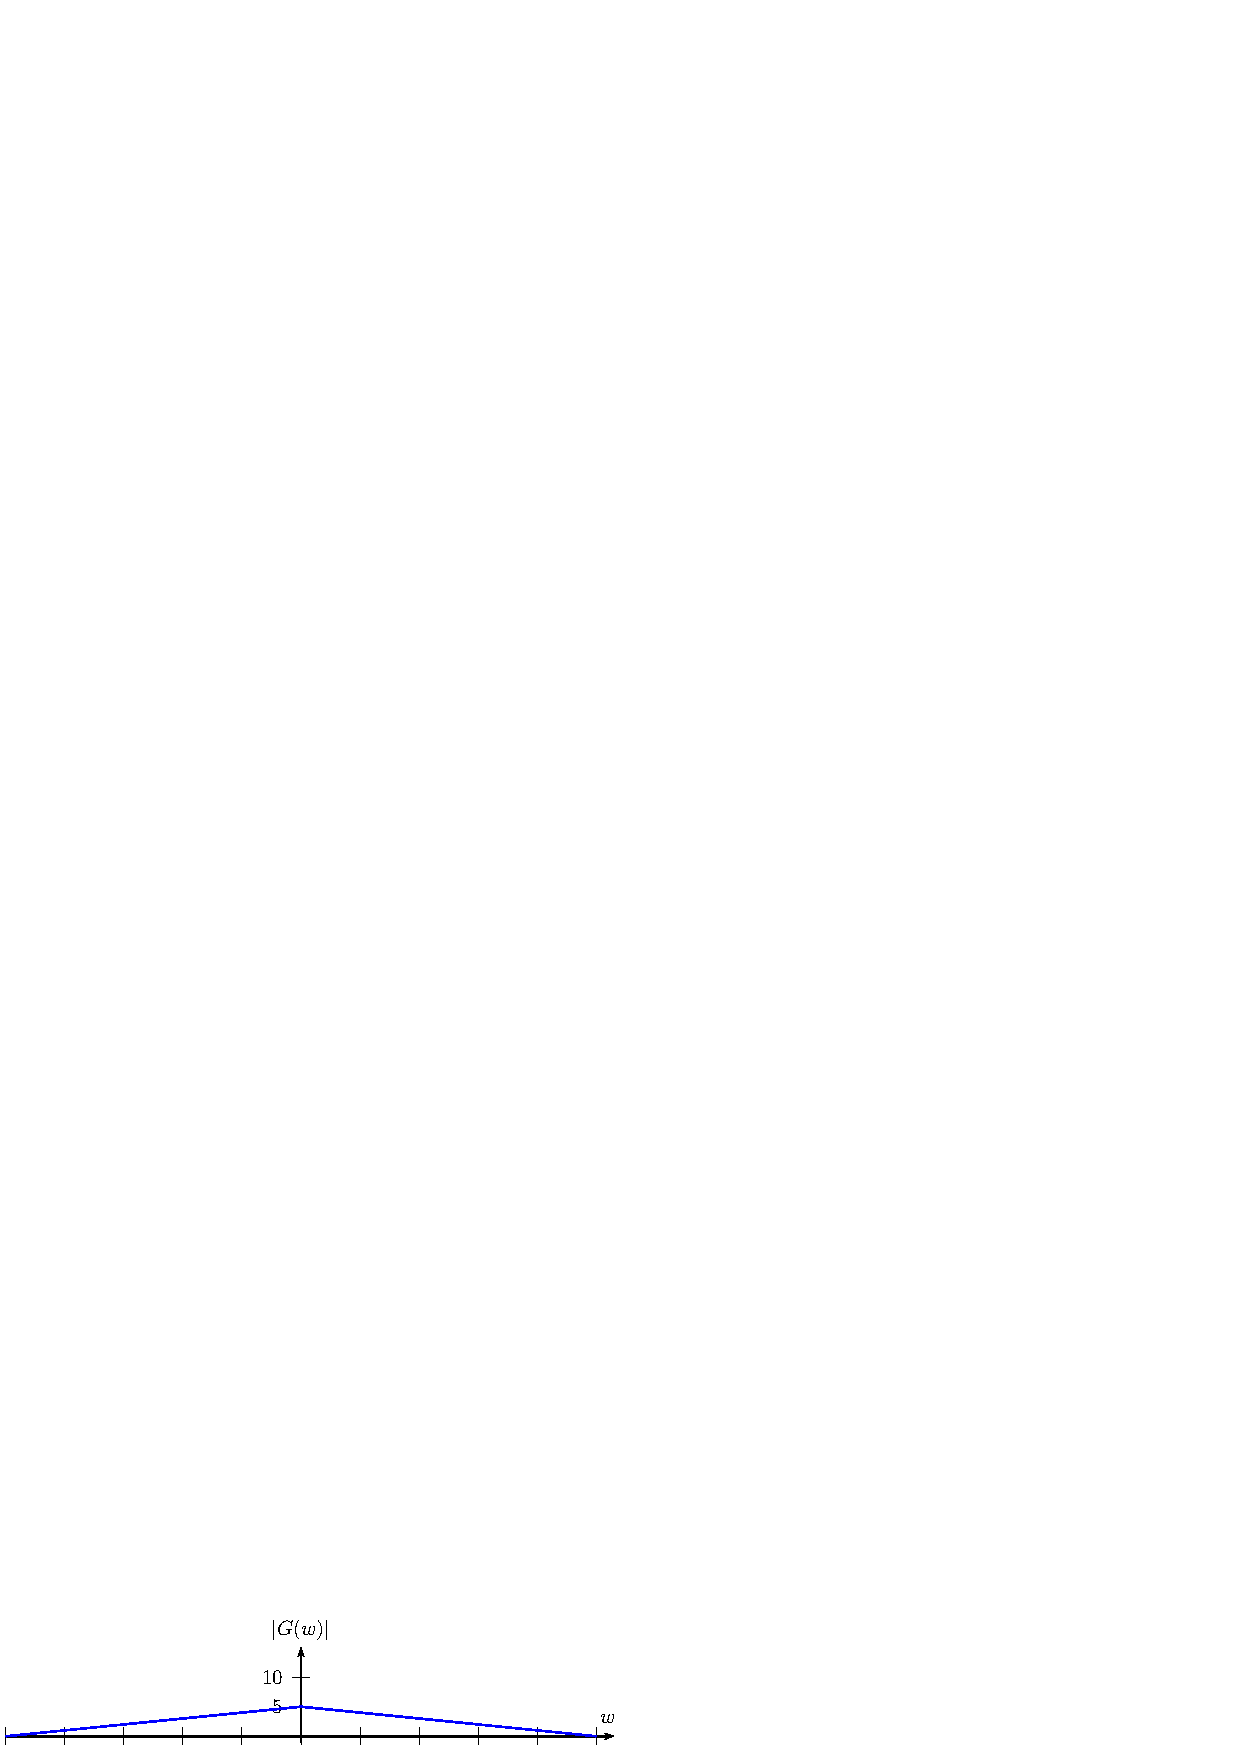
\includegraphics{cap_propriedades_transformada/pics/figura_14}\end{center}
\item[c)] 
 \begin{eqnarray*}
\mathcal{F}\left\{g(t)\right\}&=&\mathcal{F}\left\{f(-t)\right\}=F\left(-w\right)\\
\left|\mathcal{F}\left\{g(t)\right\}\right|&=&\left|F\left(-w\right)\right|=\left|\overline{F\left(w\right)}\right|=\left|F\left(w\right)\right|.
\end{eqnarray*}
Onde se usou a propriedade \ref{prop_inv_temp} e, depois, \ref{prop_conj}.
\begin{center}
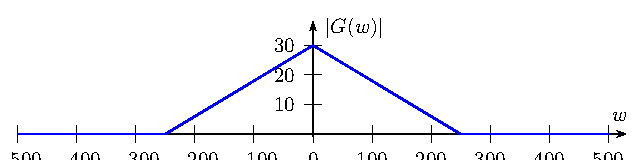
\includegraphics{cap_propriedades_transformada/pics/figura_15}\end{center}
\item[d)] 
 \begin{eqnarray*}
\mathcal{F}\left\{g(t)\right\}&=&\mathcal{F}\left\{3f(t)\right\}=3F\left(w\right)\\
\left|\mathcal{F}\left\{g(t)\right\}\right|&=&3\left|F\left(w\right)\right|.
\end{eqnarray*}
Onde se usou a propriedade \ref{prop_linear}.
\item[e)] 
 \begin{eqnarray*}
\mathcal{F}\left\{g(t)\right\}&=&\mathcal{F}\left\{f(t)\cos(1000t)\right\}\\
&=&\frac{1}{2}\left[F(w-1000)+F(w+1000)\right]\\
\end{eqnarray*}
\begin{center}
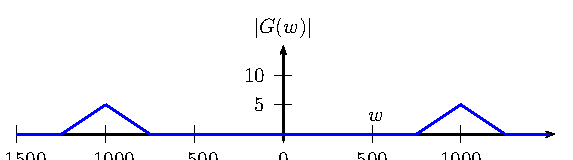
\includegraphics{cap_propriedades_transformada/pics/figura_16}\end{center}
\item[f)] 
\begin{eqnarray*}
\mathcal{F}\left\{g(t)\right\}&=&\mathcal{F}\left\{f(t)\cos^2(1000t)\right\}\\
&=&\mathcal{F}\left\{f(t)\frac{\left(1+\cos(2000t)\right)}{2}\right\}\\
&=&\frac{1}{2}F(w) + \frac{1}{4}\left[F(w-2000)+F(w+2000)\right]
\end{eqnarray*}
\begin{center}
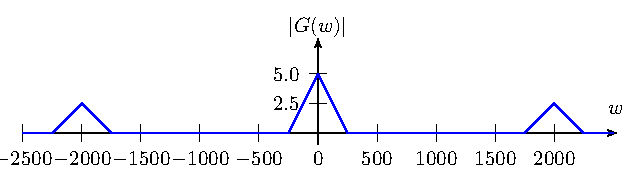
\includegraphics{cap_propriedades_transformada/pics/figura_17}\end{center}
\item[g)]
\begin{eqnarray*}
\mathcal{F}\left\{g(t)\right\}&=&\mathcal{F}\left\{f(t)\sen(1000t)\right\}\\
&=&\frac{i}{2}\left[F(w+1000)-F(w-1000)\right]\\
\end{eqnarray*}
O diagrama de magnitudes é o mesmo do item e.
\item[h)] 
\begin{eqnarray*}g(t)&=&f(t)|\sen(1000x)|\\
    &=&f(t)\left[\frac{2}{\pi}-\frac{4}{\pi}\left(\frac{\cos(2000x)}{1\cdot 3}+\frac{\cos(4000x)}{3\cdot 5}+\frac{\cos(6000x)}{5\cdot 7}+\cdots\right)\right]
\end{eqnarray*}
\begin{eqnarray*}
\mathcal{F}\{g(t)\}&=&\frac{2}{\pi}F(w)\\
&-&\frac{2}{3\pi}\left[F(w+2000)+F(w-2000)\right]\\
&-&\frac{2}{15\pi}\left[ F(w+4000)+F(w-4000)\right]\\
&-&\frac{2}{35\pi}\left[ F(w+6000)+F(w-6000)\right]+\cdots
\end{eqnarray*}
Veja o diagrama de magnitudes no gráfico abaixo.
\begin{center}
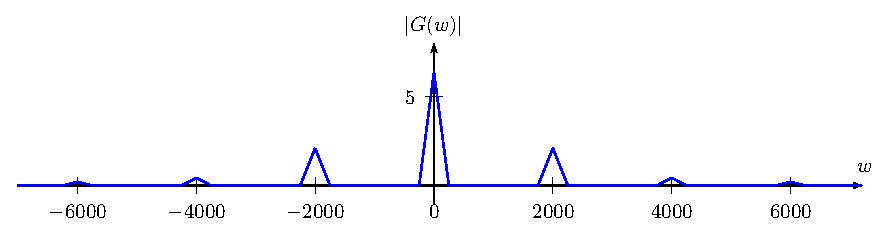
\includegraphics{cap_propriedades_transformada/pics/figura_18}\end{center}
\item[i)] Usamos a propriedade \ref{prop_der} para obter
\begin{eqnarray*}
\mathcal{F}\{g(t)\}=iwF(w).
\end{eqnarray*}
Veja o diagrama de magnitudes no gráfico abaixo.
\begin{center}
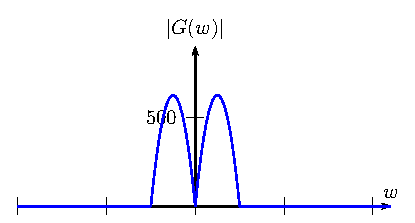
\includegraphics{cap_propriedades_transformada/pics/figura_19}\end{center}
\item[j)] 
\begin{eqnarray*}
\mathcal{F}\{g(t)\}&=&\mathcal{F}\{f(t)\ast f(t)\}=F(w)^2 \\
|G(w)|&=&|F(w)|^2.
\end{eqnarray*}
Onde se usou a propriedade da convolução  \ref{prop_teo_conv}. Veja o diagrama de magnitudes no gráfico abaixo.
\begin{center}
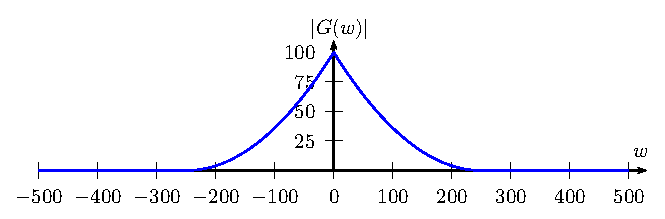
\includegraphics{cap_propriedades_transformada/pics/figura_20}\end{center}
\item[k)] 
\begin{eqnarray*}
\int_{-\infty}^\infty f(t)^2dt&=&\int_{-\infty}^\infty |f(t)|^2dt\\
&=&\frac{1}{2\pi}\int_{-\infty}^\infty |F(w)|^2dw\\
&=&\frac{1}{\pi}\int_{0}^{250} \left|10\left(1-\frac{w}{250}\right)\right|^2dw\\
&=&\frac{100}{\pi}\int_{1}^{0}  u^2\left(-250\right)du\\
&=&\frac{25000}{\pi}\int_{0}^{1}  u^2du\\
&=&\frac{25000}{\pi}\left[\frac{u^3}{3}\right]_{0}^{1}dw\\
&=&\frac{25000}{3\pi}
\end{eqnarray*}
\item[l)] 
\begin{eqnarray*}
\int_{-\infty}^\infty f(t)dt&=& F(0)\\
\left|\int_{-\infty}^\infty f(t)dt\right|&=& |F(0)|=10
\end{eqnarray*}
\end{itemize}
\end{resp}
\begin{exer} Considere o sinal $f(t)$ associado ao seguinte diagrama de espectro:
\begin{center}
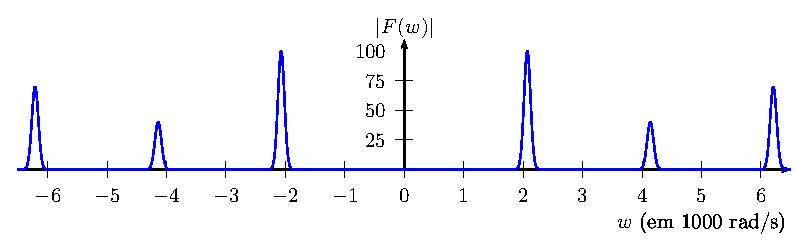
\includegraphics{cap_propriedades_transformada/pics/figura_21}\end{center}
\begin{itemize}
\item[a)] Calcule o valor de $\int_{-\infty}^\infty f(t) dt$.
\item[b)] Obtenha o valor aproximado da frequência fundamental em $Hz$ e identifique a nota.
\item[c)] Trace o diagrama de amplitudes do sinal $g(t)=\frac{f'(t)}{5000}$
\item[d)] Trace o diagrama de amplitudes do sinal $g(t)=f(-t)$.
\item[e)] Trace o diagrama de amplitudes do sinal $g(t)=f(t-2)$.
\item[f)] Trace o diagrama de amplitudes do sinal $g(t)=f(1.12t)$, obtenha o valor aproximado da frequência fundamental em $Hz$ e identifique a nota.
\item[g)] Calcule o valor da "taxa de aceleração", $a>0$, para que o sinal $g(t)=f(at)$ represente a nota sol na mesma oitava.
\end{itemize}
\end{exer}
\begin{resp}
\begin{itemize}
\item[a)] 0
\item[b)] $f_f=2070 \hbox{rad/s}=329.6 \hbox{Hz}$, equivalente à nota mi.
\item[c)] O diagrama é dada na figura abaixo.
\begin{center}
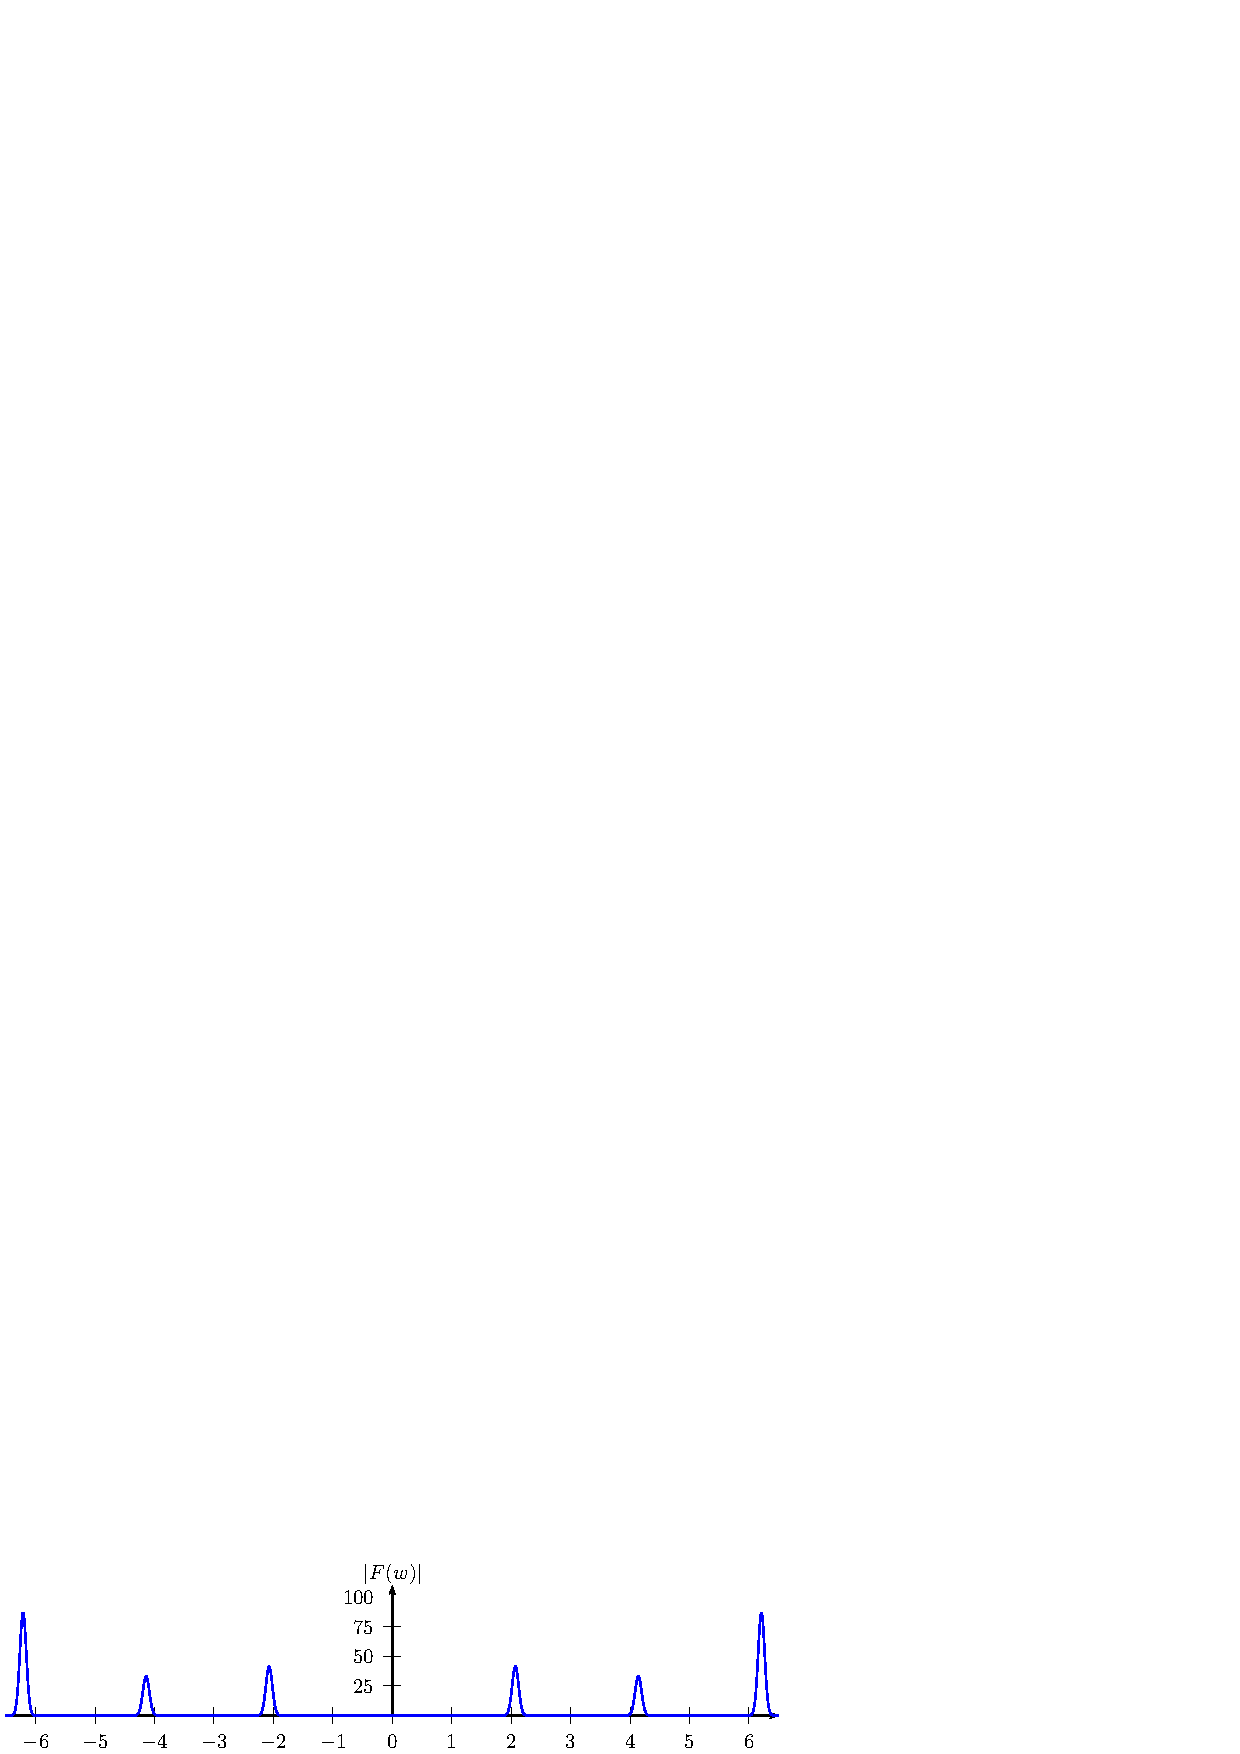
\includegraphics{cap_propriedades_transformada/pics/figura_22}\end{center}
\item[d)] Idêntico ao original.
\item[e)] Idêntico ao original.
\item[f)] Veja o diagrama abaixo.
\begin{center}
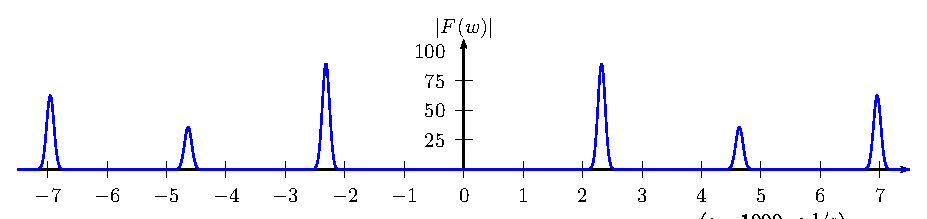
\includegraphics{cap_propriedades_transformada/pics/figura_23}\end{center}
\item[g)] \begin{equation}a=\frac{392}{329.6}=1.19\end{equation}
\end{itemize}
\end{resp}
\begin{exer} Trace o gráfico das seguintes funções, calcule sua transformada de Fourier e trace o diagrama de magnitudes: 
\begin{itemize}
\item[a)] $f(t)=e^{-|t|}\cos(10t)$.
\item[b)] $g(t)=e^{-t^2/2}\cos(10t)$.
\item[c)] $h(t)=\left\{
\begin{array}{ll}
0, &t<-4,\\
\cos(10t), &-4\leq t \leq 4,\\
0,&t>4.
\end{array} \right.$
\end{itemize}
\end{exer}
\begin{resp}
 Use o teorema da modulação. No caso c), considere $h(t)=\left[u(t-4)-u(t+4)\right]\cos(10t)$.
\end{resp}
\begin{exer} Considere uma aproximação do diagrama de espectro de magnitudes de uma nota tocada por um instrumento musical e representado por uma função $f(t)$:
\begin{center}
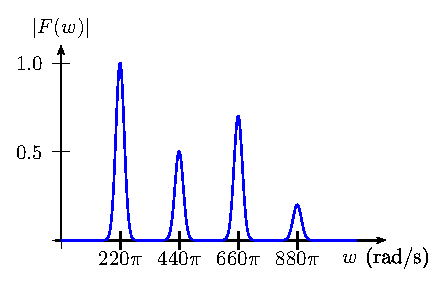
\includegraphics{cap_propriedades_transformada/pics/figura_24}\end{center}
\begin{itemize}
 \item[a)] Identifique a frequência fundamental $w_f$ (em rad/s) e $f_f$ (em Hz).
 \item[b)] Identifique a nota musical correspondente a acelerar em $1,5$ a velocidade de reprodução do sinal.
 \item[c)] Identifique a nota musical correspondente a modular o sinal na frequência $1110\pi$ rad/s ($f(t)\cos(1100\pi t)$).
 \item[d)] Identifique a nota musical correspondente à função $f(2t)$.
 \item[e)] Identifique a nota musical correspondente à função $g(t)=f(t)+f(2t)$. Qual a sensação fisiológica produzida?
 \end{itemize}
\end{exer}
\begin{resp}
\begin{itemize}
 \item[a)] $w_f=220\pi$ rad/s e $f_f=110$ Hz, equivalente ao Lá da escala 1.
 \item[b)] Mi da escala 2.
 \item[c)] Lá da escala 1.
 \item[d)] Lá da escala 2.
 \item[e)] Lá da escala 1. Percebe-se alteração na composição harmônica da nota, isto é, identicamos como uma alteração de timbre.
 \end{itemize}
\end{resp}

\section{O teorema de Parseval e o princípio da Incerteza}
\begin{teo}[Teorema de Parseval]\label{prop_teo_pars} Seja $f(t)$ uma função real ou complexa e $F(w)$ sua transformada de Fourier, então vale a identidade:
\begin{equation}\int_{-\infty}^\infty |f(t)|^2dt = \frac{1}{2\pi} \int_{-\infty}^\infty |F(w)|^2dw\end{equation}
\end{teo}
\begin{proof}
Partimos da representação de $f(t)$ em sua integral de Fourier:
\begin{eqnarray*}
f(t)=\frac{1}{2\pi}\int_{-\infty}^\infty F(w)e^{iwt}dw
\end{eqnarray*}
e consequentemente:
\begin{eqnarray*}
\overline{f(t)}=\frac{1}{2\pi}\int_{-\infty}^\infty \overline{F(w)}e^{-iwt}dw
\end{eqnarray*}
e inserimos essa expressão na integral envolvida:
\begin{eqnarray*}
\int_{-\infty}^\infty |f(t)|^2dt &=&\int_{-\infty}^\infty f(t)\overline{f(t)} dt\\
&=&\frac{1}{2\pi}\int_{-\infty}^\infty f(t)\int_{-\infty}^\infty \overline{F(w)}e^{-iwt}dw dt\\
&=&\frac{1}{2\pi}\int_{-\infty}^\infty \int_{-\infty}^\infty f(t) \overline{F(w)}e^{-iwt}dw dt\\
&=&\frac{1}{2\pi}\int_{-\infty}^\infty \int_{-\infty}^\infty f(t) \overline{F(w)}e^{-iwt}dt dw\\
&=&\frac{1}{2\pi}\int_{-\infty}^\infty \overline{F(w)}\int_{-\infty}^\infty f(t) e^{-iwt}dt dw\\
&=&\frac{1}{2\pi}\int_{-\infty}^\infty \overline{F(w)}F(w) dw\\
&=&\frac{1}{2\pi}\int_{-\infty}^\infty |F(w)|^2 dw
\end{eqnarray*}
\end{proof}
\begin{obs}Esta integral está associada ao conceito de energia total de um sinal. 
\end{obs}
\begin{ex}Considere a função $f(t)=e^{-a|t|}$, $a>0$, e sua transformada de Fourier $F(w)=\frac{2a}{w^2+a^2}$. A energia associada a essa função pode ser calculada de duas maneiras distintas:
\begin{eqnarray*}
\int_{-\infty}^\infty |f(t)|^2dt&=&\int_{-\infty}^\infty |e^{-a|t|}|^2dt\\
&=&\int_{-\infty}^\infty e^{-2a|t|}dt\\
&=&2\int_{0}^\infty e^{-2a t}dt\\
&=&2\left[-\frac{1}{2a} e^{-2a t}\right]_{0}^\infty\\
&=&\frac{1}{a}
\end{eqnarray*}
ou
\begin{eqnarray*}
\frac{1}{2\pi}\int_{-\infty}^\infty |F(w)|^2dw&=&\frac{1}{2\pi}\int_{-\infty}^\infty \left(\frac{2a}{w^2+a^2}\right)^2dw\\
&=&\frac{4a^2}{\pi}\int_{0}^\infty \frac{1}{\left(w^2+a^2\right)^2}dw
\end{eqnarray*}
Usando o item 19 da tabela de integrais definidas \ref{tab_int_def} da página \pageref{tab_int_def} com $m=0$, temos:
\begin{eqnarray*}
\int_{0}^\infty \frac{1}{\left(w^2+a^2\right)^2}dw=\frac{\pi}{4a^3}.
\end{eqnarray*}
Portanto,
\begin{eqnarray*}
\frac{1}{2\pi}\int_{-\infty}^\infty |F(w)|^2dw=\frac{4a^2}{\pi}\frac{\pi}{4a^3}=\frac{1}{a}.
\end{eqnarray*}
\end{ex}
\begin{teo}[Princípio da Incerteza*]\label{prop_princ_incert} Seja $f(t)$ uma função real que satisfaz $\lim_{t\to\pm\infty}f(t)=0$ e $F(w)=\mathcal{F}\{f(t)\}$ sua transformada de Fourier. Então vale a seguinte estimativa:
\begin{eqnarray*}
\int_{-\infty}^\infty  | tf(t)|^2dt\cdot \int_{-\infty}^\infty \left|w F(w)\right|^2dw\geq \frac{\pi}{2}
\left|\int_{-\infty}^\infty |f(t)|^2dt\right|^2 
\end{eqnarray*}
\end{teo}
\begin{proof}
Primeiro observamos que
\begin{eqnarray*}
\int_{-\infty}^\infty |f(t)|^2dt = \int_{-\infty}^\infty f(t) \overline{f(t)}dt
\end{eqnarray*}
Procedemos com intregação por partes onde $u(t)=f(t) \overline{f(t)}$, $du(t)=f'(t) \overline{f(t)}+f(t) \overline{f'(t)}$, $v(t)=t$ e $dv(t)=dt$.
\begin{eqnarray*}
\int_{-\infty}^\infty |f(t)|^2dt &=& -\int_{-\infty}^\infty t\left(f'(t) \overline{f(t)}+f(t) \overline{f'(t)}\right)dt\\
&=&-\int_{-\infty}^\infty tf'(t) \overline{f(t)}dt-\int_{-\infty}^\infty tf(t) \overline{f'(t)}dt\\
\end{eqnarray*}
Usando a desigualdade de Cauchy-Schwarz\footnote{$\left|\int f(x)g(x)dx\right|\leq \left[\int|f(x)|^2dx \cdot \int|g(x)|^2dx\right]^{1/2} $} temos
\begin{eqnarray*}
\left|\int_{-\infty}^\infty |f(t)|^2dt\right| &\leq &\left|\int_{-\infty}^\infty t \overline{f(t)} f'(t)dt\right|+\left|\int_{-\infty}^\infty tf(t) \overline{f'(t)}dt\right|\\
&\leq &\left[\int_{-\infty}^\infty  | t\overline{f(t)}|^2dt\cdot \int_{-\infty}^\infty  | f'(t)|^2dt\right]^{1/2}+\left[\int_{-\infty}^\infty  | tf(t)|^2dt\cdot \int_{-\infty}^\infty  | \overline{f'(t)}|^2dt\right]^{1/2}\\
&=&2\left[\int_{-\infty}^\infty  | tf(t)|^2dt\cdot \int_{-\infty}^\infty  | f'(t)|^2dt\right]^{1/2}.
\end{eqnarray*}
Agora, usando o teorema de Parseval (ver propriedade \ref{prop_teo_pars}), temos
\begin{eqnarray*}
\left|\int_{-\infty}^\infty |f(t)|^2dt\right|^2 &\leq & 4\int_{-\infty}^\infty  | tf(t)|^2dt\cdot \int_{-\infty}^\infty  | f'(t)|^2dt\\
&=&4\int_{-\infty}^\infty  | tf(t)|^2dt\cdot \frac{1}{2\pi}\int_{-\infty}^\infty \left|\mathcal{F}\left\{ f'(t)\right\}\right|^2dw\\
&=&\frac{2}{\pi}\int_{-\infty}^\infty  | tf(t)|^2dt\cdot \int_{-\infty}^\infty \left|iw F(w)\right|^2dw\\
\end{eqnarray*}
e, finalmente,
\begin{eqnarray*}
\int_{-\infty}^\infty  | tf(t)|^2dt\cdot \int_{-\infty}^\infty \left|w F(w)\right|^2dw \geq \frac{\pi}{2}
\left|\int_{-\infty}^\infty |f(t)|^2dt\right|^2 
\end{eqnarray*}
\end{proof}
%\subsection*{Exercícios}


\section{Passagem do contínuo para o discreto}
Nesta seção vamos calcular a transformada de Fourier de uma função periódica $f(t)$ que possui representação em série de Fourier. Para esse propósito, observe que, colocando $F(w)=2\pi \delta(w-w_0)$, temos 
\begin{equation*}
f(t)=\mathcal{F}^{-1}\{2\pi\delta(w-w_0)\}=\frac{2\pi}{2\pi}\int_{-\infty}^\infty \delta(w-w_0)e^{iwt}dw=e^{iw_0t}.
\end{equation*}
ou seja,
\begin{equation}{\label{eq_prop_trans_01}}
\mathcal{F}\{e^{iw_0t}\}=2\pi\delta(w-w_0).
\end{equation}
Agora, considere uma função $f(t)$ que possui representação em série de Fourier:
\begin{equation}
f(t)=\sum_{n=-\infty}^\infty C_n e^{iw_nt}.
\end{equation}
A definição de transformada de Fourier nos dá:
\begin{eqnarray*}
\mathcal{F}\{f(t)\}&=&\int_{-\infty}^\infty f(t) e^{-iwt}dt\\
&=&\int_{-\infty}^\infty\left( \sum_{n=-\infty}^\infty C_n e^{iw_nt}\right) e^{-iwt}dt\\
&=& \sum_{n=-\infty}^\infty C_n \left(\int_{-\infty}^\infty e^{iw_nt}e^{-iwt} dt \right)\\
&=&2\pi \sum_{n=-\infty}^\infty C_n \delta(w-w_n) ,
\end{eqnarray*}
onde usamos a equação (\ref{eq_prop_trans_01}) na última passagem.
\begin{ex}{\label{ex_ant}} Dada a função $f(t)=\cos(w_0t)$, sua representação em série trigonométrica exponencial é
\begin{equation}
f(t)=\frac{1}{2}e^{w_0it}+\frac{1}{2}e^{-w_0it}.
\end{equation}
Logo, a sua transformada de Fourier $F(w)$ é dada por:
\begin{equation}
F(w)=\pi\delta(w-w_0)+\pi\delta(w+w_0)
\end{equation}
\end{ex}
\begin{ex} Considere a função não periódica $g(t)=e^{-a|t|}\cos(w_0 t)$, $a>0$. A transformada de Fourier de $g(t)$ é dada por $G(w)=\frac{a}{(w-w_0)^2+a^2}+\frac{a}{(w+w_0)^2+a^2}$ (ver exemplo (\ref{ex_prop_trans_1.0})). Observe que 
\begin{equation}
\lim_{a\to 0}g(t)=\lim_{a\to 0} e^{-a|t|}\cos(w_0 t)=\cos(w_0 t).
\end{equation}
Comparando com o exemplo \ref{ex_ant}, é esperado que $G(w)$ convirja para $F(w)$. De fato, observe que a área abaixo da curva é constante com respeito a $a$:
\begin{eqnarray*}
\int_{-\infty}^\infty G(w)dw&=&a\int_{-\infty}^\infty \left(\frac{1}{(w-w_0)^2+a^2}+\frac{1}{(w+w_0)^2+a^2}\right)dw\\
&=&a\left[\frac{1}{a}\tan^{-1}\left(\frac{w-w_0}{a}\right)+\frac{1}{a}\tan^{-1}\left(\frac{w+w_0}{a}\right)\right]_{-\infty}^\infty\\
&=&\frac{\pi}{2}-\left(-\frac{\pi}{2}\right)+\frac{\pi}{2}-\left(-\frac{\pi}{2}\right)=2\pi
\end{eqnarray*}
e a curva $G(w)$ converge para 0, exceto em $w=w_0$ e $w=-w_0$. Portanto o limite de $G(w)$ é $F(w)$. Os diagramas de magnitude de $F(w)$ e de $G(w)$ para alguns valores de $a>0$ e $w_0=1$ são apresentados na figura \ref{diag_espec_05}.
\begin{figure}[!ht]
\begin{center}
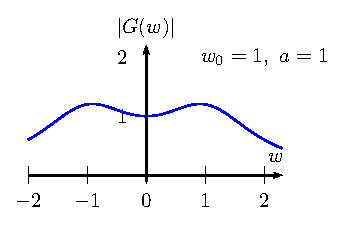
\includegraphics[width=.48\textwidth]{cap_propriedades_transformada/pics/figura_4}
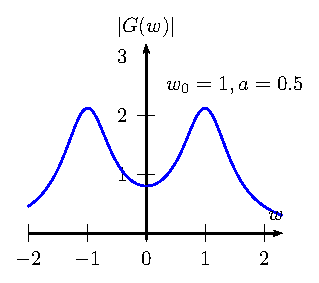
\includegraphics[width=.48\textwidth]{cap_propriedades_transformada/pics/figura_5}\vspace{30pt}
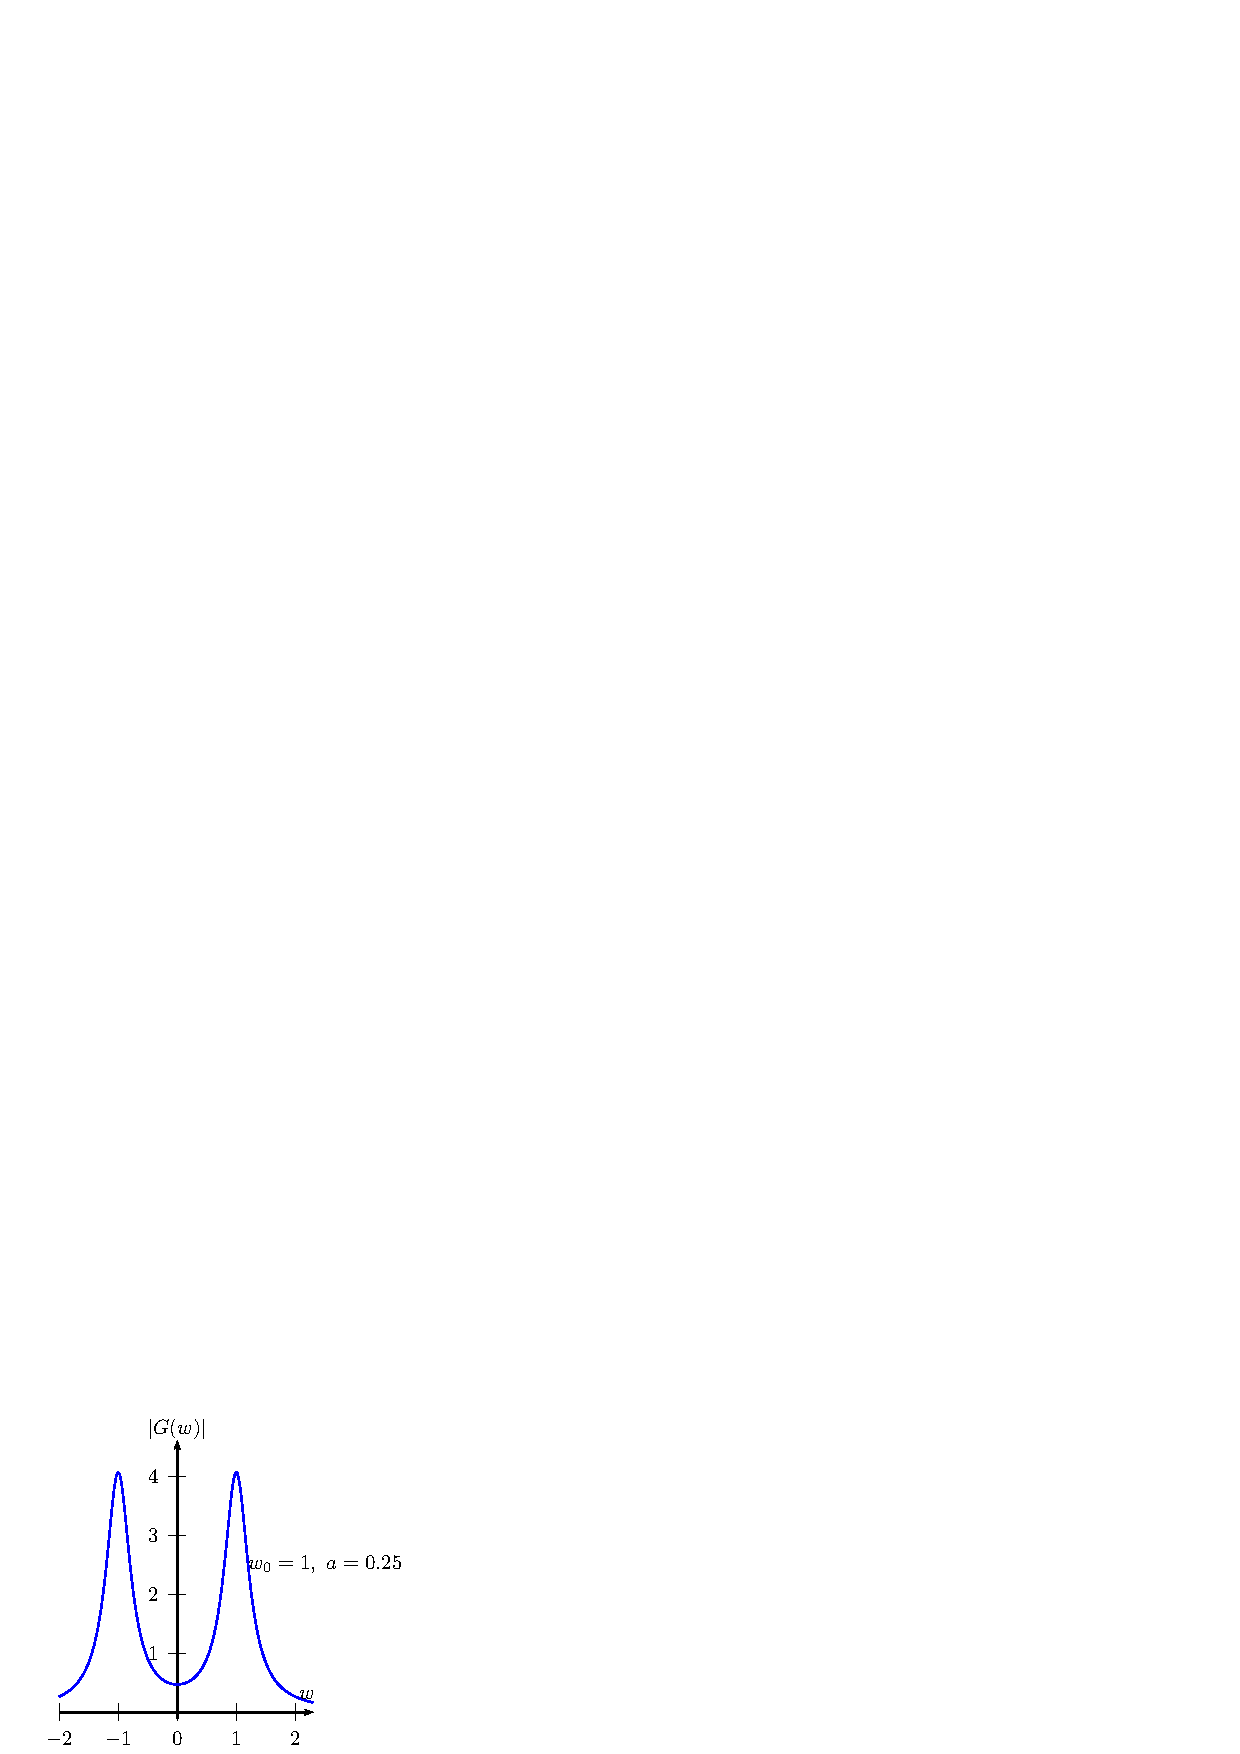
\includegraphics[width=.48\textwidth]{cap_propriedades_transformada/pics/figura_6}
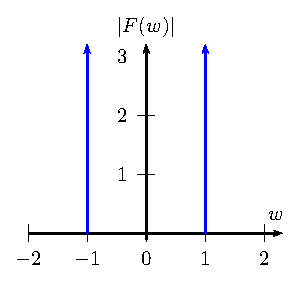
\includegraphics[width=.48\textwidth]{cap_propriedades_transformada/pics/figura_7}
\end{center}
\caption{\label{diag_espec_05}}
\end{figure}
\end{ex}~


\section{Aplicação: Sinais Discretos}
Nessa seção vamos discutir sobre discretização de sinais, em especial, pretendemos responder com que frequência precisamos amostrar um sinal real para podermos reconstruí-lo. Vamos considerar que o espectro da função $f(t)$ é composto apenas por frequências inferiores a $w_c$, onde $w_c$ é chamado de frequência de corte. Mostraremos que se conhecermos apenas os valores de $f(t)$ para $t=kT$, $k\in\mathbb{Z}$, onde $T$ é o período de amostragem e $w_a:=\frac{2\pi }{T}>2w_c$  é a frequência de amostragem, então podemos reconstruir exatamente $f(t)$ em todos instantes de tempo.
Considere $f(t)$ uma função real, definiremos $f_T(t)$ uma versão discretizada deste sinal da seguinte forma:
\begin{equation}
f_T(t)=\sum_{k=-\infty}^\infty f(kT) \delta (t-kT),
\end{equation}
assim $f_T(t)$ é um trem de Dirac, cujas amplitudes coincidem com o valor da função $f(t)$ nos pontos de amostragem $kT$. Veja um exemplo na figura \ref{sinal_discreto}.
\begin{figure}[!ht]
\begin{center}
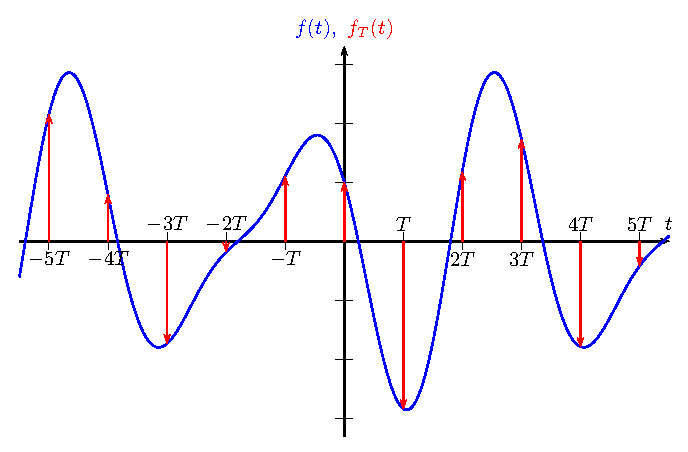
\includegraphics[width=\textwidth]{cap_propriedades_transformada/pics/figura_8}\end{center}
\caption{\label{sinal_discreto}}
\end{figure}
A fim de calcularmos a transformada de Fourier de $f_T(t)$, observamos que:
\begin{eqnarray*}
f_T(t)&=&\sum_{k=-\infty}^\infty f(kT) \delta (t-kT)\\
&=&\sum_{k=-\infty}^\infty f(t) \delta (t-kT)\\
&=&f(t)\sum_{k=-\infty}^\infty \delta (t-kT)\\
&=&f(t)\delta_T(t)
\end{eqnarray*}
onde $\delta_T(t)=\sum_{k=-\infty}^\infty \delta (t-kT)$ é uma função periódica cuja série de Fourier é dada por:
\begin{equation}\delta_T(t)=\sum_{k=-\infty}^\infty \delta (t-kT)=\sum_{n=-\infty}^\infty C_n e^{iw_n t}\end{equation}
e
\begin{equation}C_n=\frac{1}{T}\int_{-T/2}^{T/2}\delta_T(t) e^{-iw_n t}dt=\frac{1}{T}\end{equation}
assim,
\begin{equation}\delta_T(t)=\frac{1}{T}\sum_{n=-\infty}^\infty  e^{iw_n t}\end{equation}
e, portanto:
\begin{eqnarray*}
f_T(t)&=&f(t)\delta_T(t)\\
&=& f(t)\frac{1}{T}\sum_{n=-\infty}^\infty  e^{iw_n t}\\
&=&\frac{1}{T}\sum_{n=-\infty}^\infty f(t) e^{iw_n t}
\end{eqnarray*}
e finalmente:
\begin{eqnarray*}
F_T(w)&=&\mathcal{F}\left\{f_T(t)\right\}\\
&=&\frac{1}{T}\mathcal{F}\left\{\sum_{n=-\infty}^\infty f(t) e^{iw_n t}\right\}\\
&=&\frac{1}{T}\sum_{n=-\infty}^\infty F(w-w_n)
\end{eqnarray*}
onde se usou a propriedade do deslocamento no eixo $w$ (\ref{prop_desl_w}). Veja um exemplo na figura \ref{sinal_discreto1}.
\begin{figure}[!ht]
\begin{center}
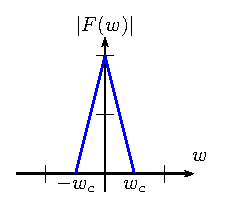
\includegraphics[width=.2\textwidth]{cap_propriedades_transformada/pics/figura_9}\vspace{10pt}
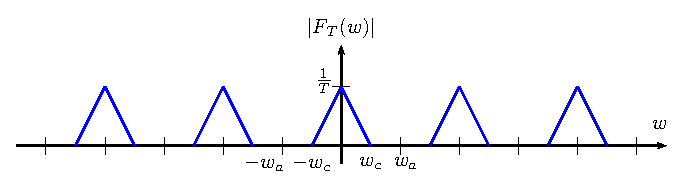
\includegraphics[width=\textwidth]{cap_propriedades_transformada/pics/figura_10}\end{center}
\caption{\label{sinal_discreto1}}
\end{figure}
\begin{obs}Observamos que se a frequência de amostragem $w_a$ for superior a $2w_c$, então $F_T(w)=\frac{1}{T}F(w)$ no intervalo $[-w_c,w_c]$ e, portanto, toda a informação de $f(t)$ é preservada. De fato, neste caso, podemos escrever:
\begin{eqnarray*}
f(t)&=&\frac{1}{2\pi}\int_{-\infty}^\infty F(w)e^{iwt}dw\\
&=&\frac{1}{2\pi}\int_{-w_c}^{w_c} F(w)e^{iwt}dw\\
&=&\frac{1}{2\pi}\int_{-w_c}^{w_c} TF_T(w)e^{iwt}dw
\end{eqnarray*}
Como $F_T(w)$ pode ser calculada apenas com base nos pontos de amostragem, $f(t)$ pode ser reconstruída. Se $w_a<2w_c$, então existe superposição espectral, o que impede a reconstrução da $f(t)$. Este resultado é conhecido como teorema da amostragem de Nyquist-Shannon ou teorema cardinal da interpolação.
\end{obs}
\begin{teo} Suponha que $f(t)$ é uma função real cujo espectro é limitado pela frequência $w_c$, isto é, $F(w)=0$ se $|w|>w_c$, e $T<\frac{\pi}{w_c}$, então
\begin{equation}
f(t)=\sum_{n=-\infty}^\infty f(nT) \frac{2\sen\left(\frac{w_a}{2}(t-nT)\right)}{w_a(t-nT)}
\end{equation}
\end{teo}
\begin{proof} Seja $F_T(w)$ a transformada de Fourier do sinal amostrado, conforme vimos, vale a expressão:
\begin{equation}
TF_T(w)=\sum_{n=-\infty}^\infty F(w-w_n).
\end{equation}
Observe que $TF_T(w)$ é uma função periódica de período $w_a$ (veja figura \ref{sinal_discreto1}), de forma que $TF_T(w)$ admite uma representação em série de Fourier:
\begin{equation}
TF_T(w)=\sum_{-\infty}^\infty D_n e^{iv_n w}=\sum_{-\infty}^\infty D_n e^{in Tw},
\end{equation}
onde usamos que $v_n=\frac{2\pi n}{w_a}=Tn$ e 
\begin{eqnarray*}
D_n&=&\frac{1}{w_a}\int_{-w_a/2}^{w_a/2}TF_T(w)e^{-in Tw}dw\\
&=&\frac{1}{w_a}\int_{-w_a/2}^{w_a/2}F(w)e^{-in Tw}dw\\
&=&\frac{1}{w_a}\int_{-\infty}^{\infty}F(w)e^{-in T w}dw,\quad \hbox{pois}\ F(w)=0\ \hbox{se}\ |w|>\frac{w_a}{2}>w_c\\
&=&\frac{2\pi}{w_a}f(-nT)=Tf(-nT),\quad \hbox{usando a transformada inversa}.
\end{eqnarray*}
Logo,
\begin{equation}
TF_T(w)=T\sum_{n=-\infty}^\infty f(-nT) e^{in Tw}.
\end{equation}
Usando a transformada inversa, temos:
\begin{eqnarray*}
f(t)&=&\frac{1}{2\pi}\int_{-w_a/2}^{w_a/2}TF_T(w) e^{i w t}dw\\
&=&\frac{1}{2\pi}\int_{-w_a/2}^{w_a/2}T\sum_{n=-\infty}^\infty f(-nT) e^{in Tw} e^{i w t}dw\\
&=&\frac{T}{2\pi}\int_{-w_a/2}^{w_a/2}\sum_{n=-\infty}^\infty f(-nT) e^{iw(t+nT)} dw\\
&=&\frac{1}{w_a}\sum_{n=-\infty}^\infty f(-nT)\int_{-w_a/2}^{w_a/2}  e^{iw(t+nT)} dw\\
&=&\frac{1}{w_a}\sum_{n=-\infty}^\infty f(-nT)\int_{-w_a/2}^{w_a/2}  \cos(w(t+nT)) dw,\quad \hbox{pois o seno é ímpar}\\
&=&\frac{1}{w_a}\sum_{n=-\infty}^\infty f(-nT)\left[  \frac{\sen(w(t+nT))}{t+nT} \right]_{-w_a/2}^{w_a/2}\\
&=&\sum_{n=-\infty}^\infty f(-nT) \frac{2\sen\left(\frac{w_a}{2}(t+nT)\right)}{w_a(t+nT)} 
\end{eqnarray*}
Substituindo $n$ por $-n$ obtemos a expressão:
\begin{equation}
f(t)=\sum_{n=-\infty}^\infty f(nT) \frac{2\sen\left(\frac{w_a}{2}(t-nT)\right)}{w_a(t-nT)}.
\end{equation}
\end{proof}



